

\newpage
\section{7-02-2019}
\par
Quali sono i tipi che risolvono il mio problema? \newline
Nei linguaggi ad oggetti, lo strumento più potente è la classe. Quando definisco le entità
che poi vado a tramutare in classi sto definendo DATI. \newline
Prima di dire cosa faranno, vado a definire chi sono. \newline
Le classi possono contenere dei metodi (funzioni che operano sugli oggetti della classe). \newline
Definire sottoclassi significa definire sottoinsiemi nell'ambito dell'ereditarietà. Le nuove operazioni delle sottoclassi vanno inserite sapendo che le sottoclassi ereditano il set di funzioni delle superclassi. \newline
L'\textit{OVERRIDING} è il punto cruciale di tutta la programmazione ad oggetti. Se non potessi farlo significa che nelle sottoclassi non posso andare a specializzare un metodo. Specializzare un metodo significa cambiare l'implementazione della super classe senza cambiarne la firma. \newline
@ serve per creare delle annotazioni nel codice, serve per il compilatore (es: @ override)
\newline
\textit{IL POLIMORFISMO} è uno strumento molto utile perchè ci permette di scrivere codice, funzioni che posso adoperare anche con tipi diversi!
\newline
\textit{DINAMIC DISPATCHING}: in fase di runtime serve a scegliere la versione giusta 
del metodo se ho degli over ride nelle mie classi. Se nella mia classe non esiste il metodo richiamato, il dinamic dispatching va a prendere l'implementazione del metodo dalla superclasse. In memoria infatti ci sono tutti i puntatori ai metodi di una classe, durante il run time viene eseguito il codice del puntatore corretto. (\textit{vedere: virtual table})
\newline
Le classi \textit{STATICHE} sono quelle classi in cui non si può fare riferimento a se stessi. (Un esempio possono essere i metodi statici). Il riferimento a \textit{this} nei metodi statici è assente. I metodi statici "appartengono" alla classe, non ad una sua istanza! Una classe statica interna non vede il riferimento this dell'altra classe. \newline
Le \textit{COLLECTION} sono delle interfacce della libreria di JAVA e non si possono costruire.
\newline

\begin{center}
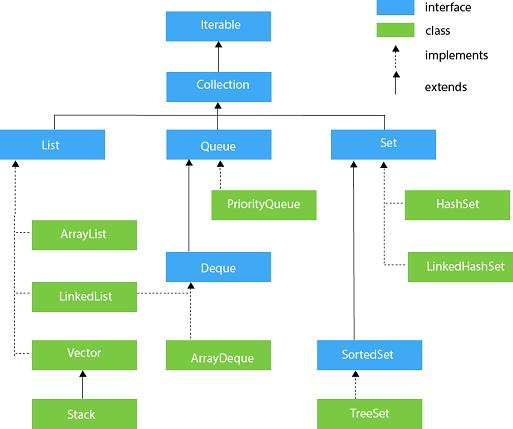
\includegraphics[width=%
0.6\textwidth]{java-collection-hierarchy}
\end{center} 

Un \textit{OGGETTO} è costituito da un insieme dei suoi campi e da puntatori ai metodi della classe $\Rightarrow$ grazie a questo il dispatching funziona, funziona perchè il compilatore ha controllato i tipi e garantisce che nel compiling time tutto questo funzioni. \newline
Ogni espressione ha un tipo!
\newline
JAVA SE $\Rightarrow$ Standard Edition \newline
JAVA EE $\Rightarrow$ Enterprise Edition \newline
JAVA ME $\Rightarrow$ Mobile Edition \newline
JAVA JDK $\Rightarrow$ linguaggio + tutte le librerie standard (java developement kit) \newline
JAVA JRE $\Rightarrow$ Solo a runtime, versione ridotta che serve solo a chi usa i programmi ma non al programmatore (java runtime enviroment) \newline
File jar  $\Rightarrow$ Archivio di tutti i pacchetti del programma \newline
JAVA JVM $\Rightarrow$ (Java virtual machine) serve per eseguire i file .jar \newline
La documentazione di java si trova on-line ed è diffusa in pacchetti che servono ad organizzare logicamente le classi, che sono organizzate in ordine alfabetico. \newline
Le \textit{COLLECTION} da sole non sono dei tipi, le collection di un "qualcosa" sono dei tipi.I tipi parametrici vogliono infatti un \textit{argomento}




\newpage










